\documentclass[11pt]{article}
\usepackage{amsmath, amssymb, amsthm}
\usepackage[retainorgcmds]{IEEEtrantools}

\usepackage{tikz}

\usepackage{fancyhdr}

%Format stuff
\pagestyle{fancy}
\headheight 35pt

%Header info
\chead{\Large \textbf{Sorting Complexity}}
\lhead{}
\rhead{}

\begin{document}
	Every comparison-based sort has a corresponding decision tree. Consider the following decision tree for an arbitrary sorting algorithm to sort a 3-element list \verb|[A, B, C]|.
	
	\begin{center}
	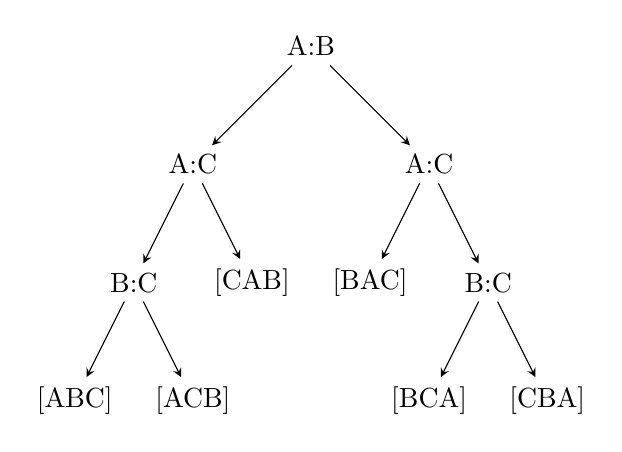
\begin{tikzpicture}
		[scale=1,line cap=round,
		%Styles
		axes/.style=,
		important line/.style={very thick},
		information text/.style={rounded corners,fill=red!10,inner sep=1ex},
		dot/.style={circle,inner sep=1pt,fill,label={#1},name=#1},
		->,>=stealth
		]
		
		%Colors
		\colorlet{anglecolor}{green!50!black}	%angle arcs/lines
		
		%The graphic
		
		\node {A:B}
			child{ node{A:C}
				child{ node{B:C} 
					child{ node{[ABC]}  }
					child{ node{[ACB]}}
				}
				child{ node{[CAB]} }
			}
			child[missing]
			child{ node{A:C}
				child{ node{[BAC]} }
				child{ node{B:C}
					child{ node{[BCA]} }
					child{ node{[CBA]} }
				}
			};
	\end{tikzpicture}
	\end{center}
	At every point in the tree, a comparison-based sort by definition will compare 2 elements. The leaves in the tree are all possible orderings for the list. For a decision tree to represent all permutations of the array, there need to be $n!$ number of leaves. For a binary decision tree there is an upper bound on the number of leaves possible:
	\begin{equation}
		L \leq 2^H
	\end{equation}
	
	Substituting $L = n!$ into the above inequality and using Stirling's Formula to expand the factorial gives
	\begin{equation}
		H \geq n\lg n + O(n)
	\end{equation}
	
	Because the height of the tree is the number of comparisons done, the optimal (lower-bound) number of comparisons for a comparison-based sort is $\Theta(n\lg n)$.
\end{document}